\section{\urwid{} 概述}
\indent\urwid{} 是为 python 设计的控制台的 UI 库. \urwid{} 可以代替库 \inlinetext{curses} 来对控制台界面进行操作, 更加便捷, 简单.%
%
\begin{figure}[!htb]
    \centering
    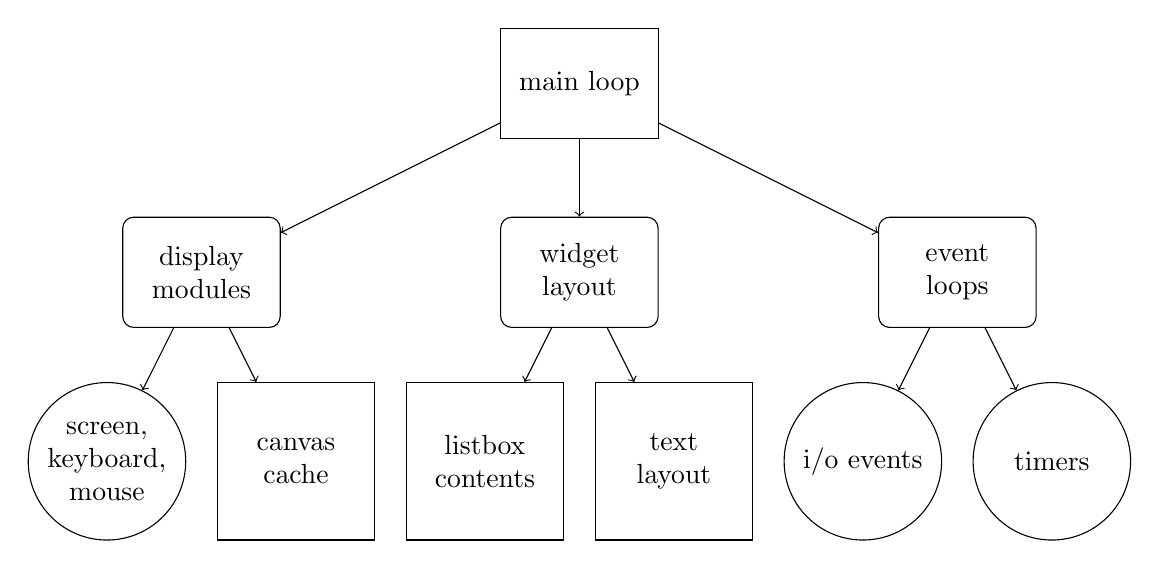
\begin{tikzpicture}[
  rectblock/.style = {rectangle, draw, inner sep = 0pt, align = flush center, minimum width = 2cm, minimum height = 1.4cm},
  roundblock/.style = {rectblock, rounded corners},
  circleblock/.style = {circle, draw, inner sep = 0pt, align = flush center, minimum size = 2cm},
  squareblock/.style = {rectblock, draw, align = flush center, inner sep = 0pt, minimum width = 2cm, minimum height = 2cm},
  x = 1.2cm,
  y = 0.8cm
]
  \node[rectblock]   (ml) at (7, 8) {main loop};
  \node[roundblock]  (dm) at (3, 5) {display\\modules};
  \node[roundblock]  (wl) at (7, 5) {widget\\layout};
  \node[roundblock]  (el) at (11, 5) {event\\loops};
  \node[circleblock] (skm) at (2, 2) {screen,\\keyboard,\\mouse}; 
  \node[squareblock] (cc) at (4, 2) {canvas\\cache};
  \node[squareblock] (lc) at (6, 2) {listbox\\contents};
  \node[squareblock] (tl) at (8, 2) {text\\layout};
  \node[circleblock] (io) at (10, 2) {i/o events};
  \node[circleblock] (ti) at (12, 2) {timers};
  
  \draw[->] (ml) -- (dm);
  \draw[->] (ml) -- (wl);
  \draw[->] (ml) -- (el);
  \draw[->] (dm) -- (cc);
  \draw[->] (dm) -- (skm);
  \draw[->] (wl) -- (lc);
  \draw[->] (wl) -- (tl);
  \draw[->] (el) -- (io);
  \draw[->] (el) -- (ti);
\end{tikzpicture}
    \caption{\urwid{} 库的结构}
    \label{fig:structure_of_urwid_library}
\end{figure}%
%
\urwid{} 的框架如\cref{fig:structure_of_urwid_library} 所示, 可见 \urwid{} 在设计之初, 就充分考虑了组件间解耦以及可扩展性.

显示模块 (display module) 负责接收用户输入, 然后将控制序列解释成键盘以及鼠标事件. 显示模块也可以用来绘制丰富的内容.

利用内置的组件可以很容易的搭建例子. 你应当把 \urwid{} 看成是一个控制台组件的集合, 而不是一个像 \inlinetext{GTK} 或是 \inlinetext{Qt} 一样的 UI 库. \urwid{} 提供的基础组件仅仅描述了它们如何在屏幕上排布.

在控制台界面中, 最多的组件就是文本 \inlinetext{Text}. \urwid{} 提供了大量的文本编码, 并且提供了一个可配置的文本布局, 可以满足大部分的对齐和断行需求. 如果你需要更加灵活的功能, 你也可以自己实现一个文本布局类.

\urwid{} 支持一些列通用显示功能, 其中包括 256 色前景色和背景色, 加粗, 下划线等等出色的显示配置. 值得注意的是, 这些功能有些终端软件并不支持, 因此, \urwid{} 可以帮助你实现一个可以自动检测终端类型并进行适配的软件.

列表框 \inlinetext{ListBox} 是 \urwid{} 中最强大的组件, 你可以用内置的遍历类也可以自己实现一个遍历类来控制列表框, 可以被用于实现列表框的滚动操作, 嵌套, 折叠以及一些类似的特性.

当组件被渲染到屏幕上的时候, 一个组件的弱引用会被保存在缓存中, 因此, 当这个组件被再次渲染的时候会特别的快. 由于是弱引用, \urwid{} 的显示模块将保持这个引用, 并用当前数据填充.

\urwid{} 的主循环简化了屏幕输入和更新的处理过程. 你也可以使用大量的事件循环, 并且支持集成 \inlinetext{Twisted} 的 Reactor 以及 \inlinetext{Glib} 的事件循环.